\subsection{RICH Detector}

The CLAS12 Ring Imaging Cherenkov Counter (RICH)~\cite{rich-nim} replaces one LTCC counter in the
Forward Detector. When charged particles traverse the aerogel radiator in the RICH volume, Cherenkov
radiation is emitted with a characteristic cone angle related to the particle velocity. These photons are
distributed in a ring pattern that can be reconstructed by collecting the photons using mirrors and PMTs
(see Fig.~\ref{Fig:RayShow} for an example RICH event). The goal of the RICH reconstruction is to provide
an estimate of the Cherenkov angle for each detected photon and intercepted particle track, to allow
subsequent particle identification. This requires input from the Forward Detector tracking service, which
defines the trajectory of particle tracks inside the detector and, in particular, the track intersection point and
direction within the aerogel radiator and the photodetector plane composed of multi-anode PMTs (MaMPTs). 

\begin{figure}[t]
\begin{center}
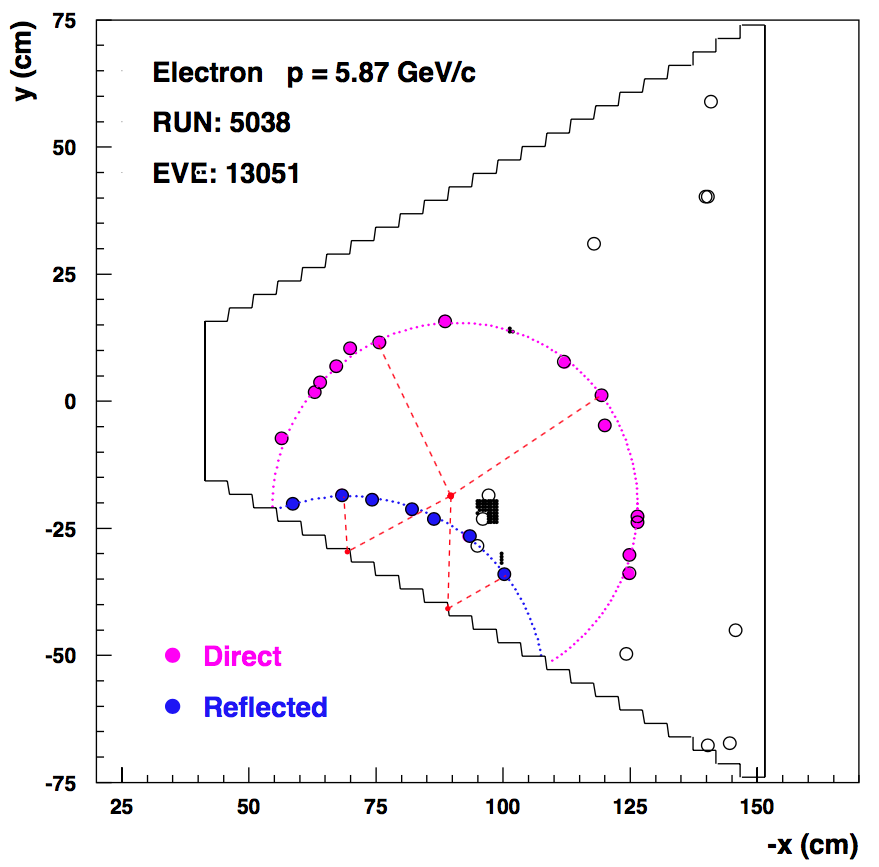
\includegraphics[width=0.8\columnwidth]{pics/example.png}
\end{center}
\caption{Example of ray-tracing from a beam event in the RICH. The open circles are the RICH detected hits and
  the circles are filled in the case that a viable traced solution has been found. The small points indicate the
  expected pattern for an electron as identified by CLAS12. The dashed lines show examples of the ray-traced
  photon paths from the common emission point (in the radiator) to the detected hit for two photons emitted
  upward that are detected directly, and two photons emitted downward that are detected after reflection from
  the mirrors. The central cluster is generated by the track impact on the MaPMT plane.}
\label{Fig:RayShow}
\end{figure}

In the first phase, the RICH reconstruction identifies the cluster of hits produced by the charged particle in
the sensor plane. The cross-talk signals (i.e. noise hits) are identified by means of an amplitude analysis, based
on the PMT signal time-over-threshold information and in conjunction with geometrical constraints. This takes
into account that a cross-talk hit should be in the proximity of a genuine hit. Hits, neither assigned to a cluster
nor flagged as cross-talk hits, are considered Cherenkov photon candidates. 

The photon path inside the RICH is then reconstructed in two complementary ways, assuming the middle point of
the particle trajectory inside the radiator as the emission point and the hit pixel coordinates as the detection
point. The first method uses an analytic formula and provides an exact solution. The formula takes into account
the refraction at the aerogel face and is only valid for directly detected photons. The second method uses a ray
tracing algorithm that takes into account also the mirror reflections. It provides a numeric solution based on a
iterative procedure. Both methods return the reconstructed Cherenkov angle in conjunction with the corresponding
aerogel refractive index, which can slightly vary with respect to the nominal value as a function of the unknown photon
energy due to chromatic effects. 

The relevant RICH components (aerogel, mirrors, MaPMT plane) are converted into ray-tracing planes or spheres
where the photon undergoes refraction, reflection, or detection. Each ray-tracing element can be independently
translated or rotated according to the results of the alignment procedure. This uses as a benchmark the Cherenkov
signal generated by electrons, as identified by other CLAS12 subsystems (ECAL, HTCC, DC). For these, the
expected Cherenkov angle is given by the known particle momentum and mass. The position and orientation of the
MaPMT plane is defined by minimizing the average distance matching the RICH clusters to the extrapolated tracks.
All other RICH ray-tracing elements can be aligned with respect to the MaPMT plane by selecting the sub-sample of
photons passing through that component. The alignment is made by minimizing the average distance between the
Ray-traced Detection Point (RdP) and the corresponding measured MaPMT hit over the selected sub-sample of
photons.

For each hadron track, the ray-tracing algorithm progresses as described in below and illustrated for an example
event in Fig.~\ref{Fig:RayShow}. A limited ensemble (of the order of 100) of hypothetical photons, called hereafter
trials, is traced assuming an initial particle hypothesis, i.e. electron for a particle identified as electron in CLAS12,
pion otherwise. A trial photon is assumed to originate at the emission point at a Cherenkov angle $\theta_T$,
corresponding to the given particle hypothesis, and at an azimuthal angle $\phi_T$, uniformly distributed around
the charged particle trajectory. For each measured MaPMT hit, the closest trial, whose RdP stays at a distance
smaller than 10~cm from the hit, is taken to be the starting point of the iterative ray-tracing procedure. At each
step, two test photons are traced by varying the trial angles by the expected angular resolution in the polar
$\theta_T \to \theta_T + \delta \theta$ and azimuthal $\phi_T \to \phi_T + \delta \phi$ directions, to quantify
the displacement of the corresponding RdP, see Fig.~\ref{Fig:RayAlgo}. The distance between the measured hit
$H$ and the trial RdP position $T$ in the sensor plane is measured in terms of the displacement of the test photon
$D$ to get an estimate of the next angular step. In particular, the scale factor $f$ of the polar angle step
$\Delta \theta = f \delta \theta$ is defined by projecting the distance vector $\vec{HT}$ onto the displacement
vector: $f=(\vec{HT}\cdot \vec {DT}) / |\vec{DT}|^2$. The same is done for the azimuthal angle $\phi$.

\begin{figure}[t]
\begin{center}
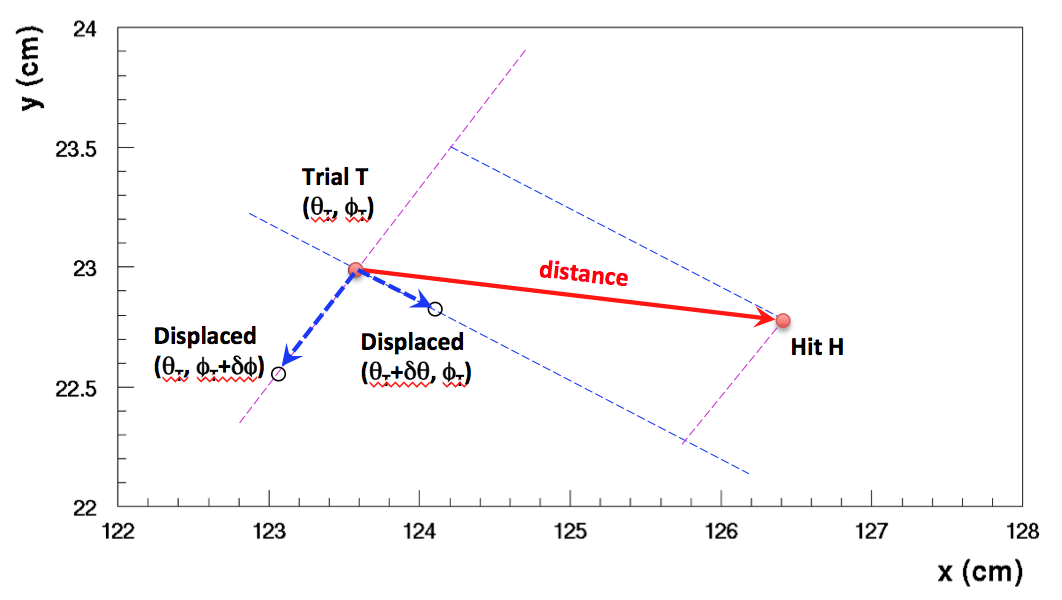
\includegraphics[width=1.0\columnwidth]{pics/ray_trace_example.png}
\end{center}
\caption{Example of the ray-tracing iterative photon path reconstruction. At each step, the polar $\theta_T$
  and azimuthal $\phi_T$ emission angles of the trial photon are varied by the expected Cherenkov angle
  resolution to extrapolate the corresponding displacements of the detection point. The distance between the
  measured hit and the trial is compared to such displacements to quantify the next angular step.}
\label{Fig:RayAlgo}
\end{figure}

A new trial photon is traced with the angles changed by such calculated angular shifts ($\theta_T + \Delta \theta$,
$\phi_T + \Delta \phi$) and the procedure repeated. At each step the trial RdP gets closer to the measured hit, but
an exact solution cannot be found as the procedure uses a linear approximation relating the distances in the MaPMT
plane with the angular steps in the 3-D space. The iterative procedure stops when the distance of the trial RdP to the
measured hit is smaller than a fraction of the MaPMT pixel size that defines the RICH detector spatial resolution.
The convergence is fast, typically within 3 steps, so that the average reconstruction time of a RICH event is 
negligible compared with that for the track reconstruction services.


